%%%%%%%%%%%%%%%%%%%%%%%%%%%%%%%%%%%%%%%%%%%%%%%%%%%%%%%%%%%%%%%%%%
%%%%%%%% NIPS 2017 EXAMPLE LATEX SUBMISSION FILE %%%%%%%%%%%%%%%%%
%%%%%%%%%%%%%%%%%%%%%%%%%%%%%%%%%%%%%%%%%%%%%%%%%%%%%%%%%%%%%%%%%%

\documentclass{article}

% use Times
\usepackage{times}
% For figures
\usepackage{graphicx} % more modern
%\usepackage{epsfig} % less modern
\usepackage{sidecap}
%\usepackage{graphics}
%\usepackage{floatrow}
\usepackage{subfigure}
\usepackage[small]{caption}
%\usepackage{subcaption}

% For side-by-side equations
\usepackage{multicol}

% Shrik the space around section headings
% \usepackage{titlesec}
% \titlespacing{\section}{0pt}{2ex}{1ex}
% \titlespacing{\subsection}{0pt}{1ex}{0ex}
% \titlespacing{\subsubsection}{0pt}{0.5ex}{0ex}
\usepackage{setspace}
\AtBeginDocument{%
  \addtolength\abovedisplayskip{-0.25\baselineskip}%
  \addtolength\belowdisplayskip{-0.25\baselineskip}%
  \addtolength\abovedisplayshortskip{-0.25\baselineskip}%
  \addtolength\belowdisplayshortskip{-0.25\baselineskip}%
}

% circled numbers
\usepackage{pifont}
\usepackage{xspace}
\newcommand{\circone}{\ding{172}\xspace}
\newcommand{\circtwo}{\ding{173}\xspace}
\newcommand{\circthree}{\ding{174}\xspace}
\newcommand{\circfour}{\ding{175}\xspace}

% For citations
\usepackage[round]{natbib}

% For appendix
\usepackage{appendix}

% Comments on equations (and algorithms)
\newcommand{\rightcomment}[1]{\(\triangleright\) {\small \it #1}}  % used to help define commands below
\newcommand{\eqcomment}[1]{\tag*{\rightcomment{#1}\quad\addtocounter{equation}{1}(\theequation)}}  % like \eqcomment* but also adds an equation number
\usepackage{suffix}
\WithSuffix\newcommand\eqcomment*[1]{\tag*{\rightcomment{#1}}}  % comment on equation within align environment

% For algorithms
\usepackage{algorithm}
%\usepackage{algorithmic}

% As of 2011, we use the hyperref package to produce hyperlinks in the
% resulting PDF.  If this breaks your system, please commend out the
% following usepackage line and replace \usepackage{icml2016} with
% \usepackage[nohyperref]{icml2016} above.
\usepackage[hidelinks]{hyperref}

% Packages hyperref and algorithmic misbehave sometimes.  We can fix
% this with the following command.
\newcommand{\theHalgorithm}{\arabic{algorithm}}

% if you need to pass options to natbib, use, e.g.:
% \PassOptionsToPackage{numbers, compress}{natbib}
% before loading nips_2017
%
% to avoid loading the natbib package, add option nonatbib:
%\usepackage[nonatbib]{nips_2017}
\usepackage[final]{nips_2017}
\makeatletter
%\renewcommand{\@noticestring}{%
%    This paper draft is under review.%
%  }
\makeatother


% improve look of algorithms (must load after icml2016!)
\usepackage[noend]{algpseudocode}
\renewcommand{\algorithmicindent}{9pt}
% hide "then" in if-statement and "do" on while-statement..
\renewcommand\algorithmicdo{:}
\renewcommand\algorithmicthen{:}
\algrenewcommand{\algorithmiccomment}[1]{\hfill \rightcomment{#1}}  % redefines \Comment (uses \rightcomment above)
\algnewcommand{\LineComment}[1]{\State \rightcomment{#1}}   % use for a whole-line comment [should improve to use parbox in case it's long]
% define \Statepar{text} command to use instead of \State when the line needs to wrap as a paragraph: http://tex.stackexchange.com/questions/200186/how-to-wrap-lines-correctly-inside-algorithmic
\makeatletter


\newcommand{\algmargin}{\the\ALG@thistlm}
\makeatother
\algnewcommand{\Statepar}[1]{\State\parbox[t]{\dimexpr\linewidth-\algmargin}{\strut #1\strut}}
% useful assignment operators
%\renewcommand{\gets}{\mathrel{:=}}
\newcommand{\pluseq}{\mathrel{+\!\!=}}

% compress spacing - from Hongyuan's friend
\setlength{\belowdisplayskip}{5.0pt} \setlength{\belowdisplayshortskip}{5.0pt}
\setlength{\abovedisplayskip}{5.0pt} \setlength{\abovedisplayshortskip}{5.0pt}
\setlength\floatsep{0.65\baselineskip}
\setlength\textfloatsep{0.65\baselineskip}
\setlength\intextsep{0.65\baselineskip}

\usepackage{xpatch}
\xapptocmd\normalsize{%  patch spacing around equations: currently this uses the ACL defaults but changes "minus 3pt" to "minus 9pt" so that latex feels comfortable squishing more
 \abovedisplayskip=11pt plus 3pt minus 9pt
 \abovedisplayshortskip=0pt plus 3pt
 \belowdisplayskip=11pt plus 3pt minus 9pt
 \belowdisplayshortskip=6.5pt plus 3.5pt minus 3pt
}{}{}

% Self-favored packages
\usepackage{amsmath}
\usepackage{amssymb}
\usepackage{mathtools, cuted} % make equations cross the two columns
% equally distribute columns in table
\usepackage{tabularx, booktabs}
\newcolumntype{C}{>{\centering\arraybackslash}X}
\newcolumntype{R}{>{\raggedleft\arraybackslash}X}
% unequally distribute columns in table
\newcolumntype{S}{>{\raggedleft\arraybackslash\hsize=.5\hsize}X}
\usepackage{latexsym}
\usepackage{url}
\usepackage{xspace}
\usepackage{bm,array}
\usepackage{amsfonts}
\usepackage{enumitem}
\usepackage{mathtools}
\usepackage{bm}
\usepackage{esvect}
\usepackage[noabbrev,capitalize]{cleveref} % to standardize references
\crefname{equation}{equation}{equations}   % "equation" is lowercased, overriding capitalize option
\crefname{section}{section}{sections}      % "section" is lowercased, overriding capitalize option
\crefname{footnote}{footnote}{footnotes}      % "section" is lowercased, overriding capitalize option
\newcommand{\crefrangeconjunction}{--}     % use -- for ranges
\usepackage{bbm} % bold for indicator function
\renewcommand{\vec}[1]{{\boldsymbol{\mathbf{#1}}}}   % requires bm package.  From http://tex.stackexchange.com/questions/3535/bold-math-automatic-choice-between-mathbf-and-boldsymbol-for-latin-and-greek
%\usepackage{unicode-math}
%\setmathfont{xits-math.otf}
\newcommand{\defn}[1]{\textbf{#1}}   % definitions
\newcommand{\defeq}{\mathrel{\stackrel{\mbox{\tiny def}}{=}}} % unicode U+225D
\DeclareMathOperator*{\argmin}{argmin}
\DeclareMathOperator*{\argmax}{argmax}
\newcommand{\E}[2][]{\mathbb{E}_{{#1}}[#2]}   % expectation
\newcommand{\Real}{\mathbb{R}}
\newcommand{\Uniform}{\mathrm{Unif}}
\newcommand{\Exp}{\mathrm{Exp}}
\renewcommand{\th}{\textsuperscript{th}\xspace}
\newcommand{\bos}{\textsc{bos}\xspace}
\newcommand{\eos}{\textsc{eos}\xspace}

% TODO NOTES
\usepackage[usenames,dvipsnames,svgnames,table]{xcolor}  % allows better color names
\usepackage[disable]{todonotes} % insert [disable] to disable all notes
%
% Note that these macros accept optional arguments such as
% size=\small, bordercolor=red, and so on.  Capitalized versions
% are inline paragraphs instead of margin notes.
\newcommand{\fixme}[2][]{\todo[color=yellow,size=\scriptsize,fancyline,caption={},#1]{#2}} % to mark stuff that you know is missing or wrong when you write the text
\newcommand{\note}[4][]{\todo[author=#2,color=#3,size=\scriptsize,fancyline,caption={},#1]{#4}} % default note settings, used by macros below
\newcommand{\jason}[2][]{\note[#1]{jason}{green!40}{#2}}
\newcommand{\hongyuan}[2][]{\note[#1]{hongyuan}{orange!40}{#2}}
\newcommand{\notewho}[3][]{\note[#1]{#2}{blue!40}{#3}}     % for other commenters: specify author name in first required arg
\newcommand{\Fixme}[2][]{\fixme[inline,#1]{#2}\noindent}
\newcommand{\Notewho}[3][]{\notewho[inline,#1]{#2}{#3}\noindent}
\newcommand{\Jason}[2][]{\jason[inline,#1]{#2}\noindent}
\newcommand{\Hongyuan}[2][]{\hongyuan[inline,#1]{#2}\noindent}

\newcommand{\cutforspace}[1]{}

% To clean:
%    latex-clean neural-hawkes --plusspace jason hongyuan fixme notewho
% Also replace \bibliography command with the contents of the .bbl file,
% and delete the cutforspace commands.

%To delete content or show the deleted part in red

% To comment out block
\usepackage{verbatim}

\title{
Parallel Training of Hawkes Process
}

% The \author macro works with any number of authors. There are two
% commands used to separate the names and addresses of multiple
% authors: \And and \AND.
%
% Using \And between authors leaves it to LaTeX to determine where to
% break the lines. Using \AND forces a line break at that point. So,
% if LaTeX puts 3 of 4 authors names on the first line, and the last
% on the second line, try using \AND instead of \And before the third
% author name.
\author{
  Hongyuan Mei	 \ \ \ \ \ \ Shjie Wu \ \ \ \ \ \ Shuo Sun\\
  Department of Computer Science, Johns Hopkins University \\
  3400 N. Charles Street, Baltimore, MD 21218 U.S.A \\
  \texttt{\{hmei,jason\}@cs.jhu.edu} \\
}

\begin{document}

\maketitle

%\input{abstract}
%%%%%%%%%
% Abstract
%%%%%%%%%
\vspace{-18pt}
\begin{abstract}
\vspace{-6pt}
Many events occur in the world. Some event types are stochastically excited---in the sense of having their probabilities elevated---by patterns in the sequence of previous events. Discovering such patterns can help us predict {\em which type} of event will happen next and {\em when}.That should benefit applications such as medical prognosis, consumer behavior, and social media activity prediction. We investigate how to train a Hawkes process in batches, thus speeding up the training procedure.
\end{abstract}

\Hongyuan{
TODO list for camera-ready:
\begin{itemize}
\item otherwise address reviewer comments
\item possibly restore bits that we cut or moved to the supplementary material for space reasons
\item connection between our many-state HMM and John Shawe-Taylor's
  ``conditional mean embeddings for RL,'' which does kernels?
\end{itemize}
}

%%%%%%%%%
% Introduction
%%%%%%%%%
\vspace{-23pt}
\section{Introduction}
\label{sec:introduction}
\vspace{-3pt}

\subsection{The Problem}
Some events in the world are correlated.  A single event, or a pattern of events, may help to cause future events.  We are interested in learning the distribution of sequences of events.  The ability to discover correlations among events is crucial to accurately predict the future of a sequence given its past, i.e., which events are likely to happen next and when they will happen.

\subsection{The Importance}
We specifically focus on sequences of discrete events in continuous time (``event streams'').
Modeling such sequences seems natural and useful in many applied domains:
\begin{itemize}
\item {\em Medical events.}  Each patient has a sequence of acute incidents, doctor's visits, tests, diagnoses, and medications.  By learning from previous patients what sequences tend to look like, we could predict a new patient's future from their past.
\item {\em Consumer behavior.}  Each online consumer has a sequence of online interactions.  By modeling the distribution of sequences, we can learn purchasing patterns.  Buying cookies may temporarily depress purchases of all desserts, yet increase the probability of buying milk.\looseness=-1
%\jason{seeing an ad may also increase the probability of buying milk: come back to this example later when we discuss causality?}
\item {\em ``Quantified self'' data.}  Some individuals use cellphone apps to record their behaviors---eating, traveling, working, sleeping, waking.\cutforspace{such as eating specific foods, traveling among locations, performing specific work and leisure activities, sleeping and waking.}  By anticipating behaviors, an app could perform helpful supportive actions, including issuing reminders\cutforspace{ or warnings} and placing advance orders.
\item {\em Social media actions.}  Previous posts, shares, comments, messages, and likes by a set of users are predictive of their future actions.
%\item {\em News events.}  In principle, we could model the single stream of publicly reported events in the world, such as business news stories and significant market events.
%\item {\em Scientific modeling.}  For example, consider a given individual's sequence of responses in a category elicitation task, ``name as many vegetables as you can think of.''  Saying {\tt squash} will prime {\tt pumpkin} but will inhibit saying {\tt squash} again.  A model of such sequences is a hypothesis about latent cognitive representations and priming mechanisms.
%\item {\em Dialogue events.} We could model topic shifts in political conversations, where one topic tends to lead quickly or slowly to another.  Or we could model the sequence of speaker-addressee pairs as characters converse in a novel, play, or online discussion.
%\item {\em Music modeling.}  We could model the sequence of notes (from one instrument or many) in a musical score or performance.
\item Other event streams arise in {\em news}, {\em animal behavior}, {\em dialogue}, {\em music}, etc.
\end{itemize}

\subsection{Related Work}
A basic model for event streams is the \defn{Poisson process}~\citep{palm-43}, which assumes that events occur independently of one another.  In a \defn{non-homogenous Poisson process}, the (infinitesimal) probability of an event happening at time $t$ may vary with $t$, but it is still independent of other events.  A \defn{Hawkes process} \citep{hawkes-71,liniger-09-hawkes}
% defines the intensity of each event as a time-variant function, but further
supposes that past events can temporarily {\em raise} the probability of future events, assuming that such excitation is \circone positive, \circtwo additive over the past events, and \circthree exponentially decaying with time.
%To train a Hawkes process, one usually adopts gradient-based methods \citep{lukasik-16-hawkes}, as the gradients can (tough very difficult to) be analytically derived out.

%%%%%%%%%
% Definition and Notation
%%%%%%%%%
\section{The Method}
\label{sec:method}
In this section, we first review Hawkes processes, and then introduce our method to train it in parallel with GPUs.

\subsection{Notation}
We are interested in constructing distributions over \defn{event streams} $(k_1,t_1), (k_2, t_2), \ldots$, where each $k_i \in \{1,2,\ldots,K\}$ is an event type and $0 < t_1 < t_2 < \cdots$ are times of occurrence. That is, there are $K$ types of events, tokens of which are observed to occur in continuous time.

For any distribution $P$ in our proposed family, an event stream is almost surely infinite.  However, when we observe the process only during a time interval $[0,T]$, the number $I$ of observed events is almost surely finite.  The {\em log-likelihood} $\ell$ of the model $P$ given these $I$ observations is
%\jason{do we really only want to do ML estimation, or should you hedge here?}
%\hongyuan{For prediction, we can also optimize the prediction accuracy like RMSE, so we can add that. But I am afraid this is a bit overwhelming. So may be we can just mention this in the section of prediction task, after we have introduced the prediction formula in section 4.}
%\jason{Prediction is after training.  I was asking whether we are going to insist on training by plain MLE, without any regularizer or prior.  Since this is the notation section, I've hedged by saying that this is the log-likelihood, without saying that maximizing it is our goal.}
\begin{equation}\label{eqn:loglik-orig}
    \Big( \sum_{i=1}^I \log P\!\left( \left(k_i,t_i\right) \mid \mathcal{H}_{i} \right) \Big) + \log P(t_{I+1} > T \mid \mathcal{H}_I)
\end{equation}
where the \defn{history} $\mathcal{H}_{i}$ is the prefix sequence $(k_1,t_1)$, $(k_2, t_2), \ldots, (k_{i-1}, t_{i-1})$, and
$P((k_i, t_i) \mid \mathcal{H}_i )\,dt$ is the probability that the {\em next} event occurs at time $t_i$ and has type $k_i$.\looseness=-1

Throughout the paper, the subscript $i$ usually denotes quantities that affect the distribution of the next event $(k_i,t_i)$. These quantities depend only on the history ${\cal H}_i$.

We use (lowercase) Greek letters for parameters related to the classical Hawkes process,
and Roman letters for other quantities, including affine transformation parameters.
We denote vectors by bold lowercase letters such as $\vec{s}$ and $\vec{\mu}$, and matrices by bold capital Roman letters such as $\vec{U}$. Subscripted bold letters denote distinct vectors or matrices (e.g., $\vec{w}_k$).
%for example, $\vec{\delta}_k$, $\vec{h}_i$ and $\vec{D}_k$.  % (to be defined in~\cref{sec:model}).
Scalar quantities, including vector and matrix elements such as $s_k$ and $\alpha_{j,k}$, are written without bold. Capitalized scalars represent upper limits on lowercase scalars, e.g., $1 \leq k \leq K$.  Function symbols are notated like their return type.
All $\Real \rightarrow \Real$ functions are extended to apply elementwise to vectors and matrices.\looseness=-1

\subsection{Hawkes Process: A Self-Exciting Multivariate Point Process}
\label{sec:poisson_process}
\label{sec:hawkes_process}
\label{sec:SE-MPP}
Formally, generative models of event streams are \defn{multivariate point processes}.  A (temporal) point process is a probability distribution over $\{0,1\}$-valued functions on a given time interval (for us, $[0,\infty)$).  A multivariate point process is formally a distribution over $K$-tuples of such functions.  The $k$\th function indicates the times at which events of type $k$ occurred, by taking value 1 at those times.

%\paragraph{Definition}
A basic model of event streams is the \defn{non-homogeneous multivariate Poisson process}.  It assumes that an event of type $k$ occurs at time $t$---more precisely, in the infinitesimally wide interval $[t,t+dt)$---with probability $\lambda_k(t) dt$.  The value $\lambda_k(t) \geq 0$ can be regarded as a rate per unit time, just like the parameter $\lambda$ of an ordinary Poisson process.  $\lambda_k$ is known as the \defn{intensity function}, and the total intensity of all event types is given by $\lambda(t) = \sum_{k=1}^K \lambda_k(t)$.

%\jason{what is a member model?  do you mean that a Hawkes process is an example of a non-homogeneous point process?}

A well-known generalization that captures interactions is the \defn{self-exciting multivariate point process (SE-MPP)},
%\jason{what does ``multivariate'' refer to?}
or \defn{Hawkes process} \citep{hawkes-71,liniger-09-hawkes}, in which past events $h$ from the history conspire to {\em raise} the intensity of each type of event.
Such excitation is positive, additive over the past events, and exponentially decaying with time:
\begin{align}\label{eqn:hawkes}
    \lambda_k(t)
    %&= \mu_k + \sum_{i: t_i < t} \nu_{k_i,k}(t-t_i)\\
    &= \mu_k + \sum_{h: t_h < t} \alpha_{k_h,k} \exp (-\delta_{k_h,k} (t-t_h) )
\end{align}
where \mbox{$\mu_{k} \geq 0$} is the base intensity of event type $k$, \mbox{$\alpha_{j,k} \geq 0$} is the degree to which an event of type $j$ initially excites type $k$, and \mbox{$\delta_{j,k} > 0$} is the decay rate of that excitation.
%\jason{shouldn't some of these be $\geq 0$ rather than $> 0$?  in fact, could the decay rate be negative for an ``explosive'' process?  Just follow tradition here, I think.}
When an event occurs, all intensities are elevated to various degrees, but then will decay toward their base rates $\vec{\mu}$.

%%%%%%%%%
% Algorithm
%%%%%%%%%
%\vspace{-4pt}
\subsection{Algorithms}
\label{sec:algo}

%\vspace{-4pt}
For the proposed model,
the log-likelihood \eqref{eqn:loglik-orig} of the parameters turns out to be given by a simple formula---the sum of the log-intensities of the events that happened, at the times they happened, minus an integral of the total intensities over the observation interval $[0,T]$:
\begin{equation}\label{eqn:loglik}
    {\ell} = \sum_{i: t_i \leq T} \log \lambda_{k_i}(t_i) - \underbrace{\int_{t=0}^{T} \lambda(t) dt}_{\text{call this }\Lambda}
\end{equation}
for which the details can be found in \cref{sec:lik}.
Intuitively, the $-\Lambda$ term (which is $\leq 0$) sums the log-probabilities of infinitely many {\em non}-events.  Why?  The probability that there was {\em not} an event of any type in the infinitesimally wide interval $[t,t+dt)$ is $1-\lambda(t)dt$, whose log is $-\lambda(t) dt$.
We can locally maximize ${\ell}$ using any stochastic gradient method. 

Plugging \cref{eqn:hawkes} into \cref{eqn:loglik} yields the formula:
\begin{equation}\label{eqn:loglik-full}
    {\ell} = \sum_{i: t_i \leq t_I} \log \lambda_{k_i}(t_i) -  T \sum_{k=1}^{K} \mu_k - \sum_{k=1}^{K} \sum_{i=1}^{I} \frac{\alpha_{k_i,k}}{\delta_{k_i,k}} ( 1 - \exp(-\delta_{k_i,k}(T-t_i)) )
\end{equation}
for which the details can be found in \cref{sec:likhawkes}.

We observe that if we can rewrite \cref{eqn:loglik} in its matrix form, we can then build a computational graph of these mathematical expressions, thus leveraging the computational efficiency by training it on many sequences in parallel on a GPU device. 

%\subsubsection{Matrix Formulation for Parallelism}
We first investigate how the likelihood function for a single sequence $(k_1,t_1), (k_2, t_2), \ldots, (k_I,t_I)$ is rewritten in its matrix form, and then extend it to mini-batch settings. 

For a single sequence, we create a matrix $\vec{T} \in \Real^{I \times I}$ such that $T_{i,j} = t_i - t_j$ if $i > j$ and $T_{i,j} = 0$ otherwise, and a mask matrix $\vec{M} \in \{0,1\}^{I \times I}$ such that $M_{i,j}=1$ if $i > j$ and $M_{i,j}=0$ otherwise. Moreover, we construct matrices $\vec{A}, \vec{D} \in \Real_{+}^{I \times K}$ by indexing $\vec{\alpha}$ and $\vec{\delta}$ respectively, such that $A_{i,k} = \alpha_{k_i, k}$ and $D_{i,k} = \delta_{k_i,k}$. This way, the vector $\vec{\lambda}(t_i)$ can be rewritten as
\begin{equation}
\vec{\lambda}(t_i) = \vec{\mu} + {\vec{1}(I)}^{\top} (\vec{M}_{i} \times \vec{1}(K)) \odot A \odot \exp{(-\vec{D} \odot (\vec{T}_i \times \vec{1}(K) ) )}
\end{equation}
where $\odot$ is elementwise multiplication, $\times$ is outer product, and $\vec{1}(D)$ is a $D$-dimensional one vector. . So the summation of log intensities term in \cref{eqn:loglik-full} can be easily constructed by indexing the $k_i$-th entry in each $\vec{\lambda}(t_i)$ and summing their logarithms. 

The second term, $-T \sum_{k=1}^{K} \mu_k$ is trivial to be converted into its matrix form $T \vec{\mu}^\top \vec{1}$ 

Similar to the first term, the matrix form of the last term in \cref{eqn:loglik-full} can also be constructed as:
\begin{equation}
\vec{1}(I) ( \frac{\vec{D}}{\vec{A}} (\vec{1}(I,K) - \exp(-\vec{D} \odot (\vec{T}_{I} \times \vec{1}(K) ) )) ) \vec{1}(K)
\end{equation}
where $\vec{1}(I,K)$ denotes a one matrix of shape $I \times K$. 

After constructing the matrix form of the log-likelihood function for one sequence, it is trivial to extend the tensors by one extra dimension and stack the computation for all the sequences in one mini-batch into one tensor. 

Why this is important? Because in this way, we can build its computational graph by writing down this matrix form expression in any existing graph-based scientific computing libraries like Theano and PyTorch, and get two advantages:
\begin{itemize}
\item Gradients are automatically taken care of by the library so we do not have to manually compute any derivative; 
\item It is easy to use GPUs this way, because GPU's cores are naturally well-suited for matrix computation. 
\end{itemize}

%%%%%%%%%
% Experimental Details
%%%%%%%%%
%\newpage
\section{Experiments}
\label{sec:experiments}

In this section, we elaborate on the details of experiments.

\subsection{Dataset}
\label{sec:data_stats}
We evaluate our method on one simulated dataset.
The sequences were generated by a randomly initialized Hawkes process with {Thinning algorithm} \citep{liniger-09-hawkes}.
Dataset details can be found in~\cref{tab:stats_dataset} and sequences sampling details can be found in \cref{sec:thinning}. 

Why do we have to use sampled data, rather than any real-world data? Because we would like to make sure our matrix-form expression and implementation is correct! This can be done by checking whether the same set of parameters can yield exactly the same log-likelihood results on the same set of sampled sequences regardless of the formulation and implementation. 

\begin{table*}[t]
\begin{center}
\begin{small}
\begin{sc}
%\begin{tabularx}{1.00\textwidth}{l *{1}{R}*{6}{R}}
\begin{tabularx}{1.00\textwidth}{l *{1}{S}*{3}{R}*{3}{S}}
%\begin{tabularx}{0.95\textwidth}{lc rrr rrrr}
\toprule
%Dataset & \multicolumn{1}{c}{\# of Event Types} & \multicolumn{3}{c}{\# of Event Tokens} & \multicolumn{3}{c}{Sequence Length} \\
Dataset & \multicolumn{1}{r}{$K$} & \multicolumn{3}{c}{\# of Event Tokens} & \multicolumn{3}{c}{Sequence Length} \\
\cmidrule(lr){3-8}
  &  & Train & Dev & Test & Min & Mean & Max \\
\midrule
%Synthetic (SE-MPP) & $5$ & $482947$ & $59683$ & $60067$ & $20$ & $60.27$ & $100$ \\
%Synthetic (D-SM-MPP) & $5$ & $480219$ & $60380$ & $59638$ & $20$ & $60.02$ & $100$ \\
%Synthetic (N-SM-MPP) & $5$ & $478182$ & $60407$ & $60712$ & $20$ & $59.93$ & $100$ \\
%Synthetic & $5$ & $\approx 480449$ & $\approx 60217$ & $\approx 60139$ & $20$ & $\approx 60$ & $100$ \\
Synthetic & $5$ & $160449$ & $20217$ & $20139$ & $10$ & $20$ & $30$ \\
%Retweets & $3$ & $1739547$ & $215521$ & $218465$ & $50$ & $109$ & $264$ \\
%MemeTrack & $5000$ & $93267$ & $14932$ & $15440$ & $1$ & $3$ & $31$ \\
%MIMIC-II & $75$ & $\approx 1946$ & $\approx 228$ & $\approx 245$ & $2$ & $4$ & $33$ \\
%StackOverflow & $22$ & $\approx 343998$ & $\approx 39247$ & $\approx 97168$ & $41$ & $72$ & $736$ \\
%Financial & $2$ & $\approx 298710$ & $\approx 33190$ & $\approx 82900$ & $829$ & $2074$ & $3319$ \\
\bottomrule
\end{tabularx}
\end{sc}
\end{small}
\end{center}
%\vspace{-10pt}
 \caption{
 	Statistics of each dataset. 
}
\label{tab:stats_dataset}
%\Hongyuan{merge first 3 rows, using $\approx$}
%\Hongyuan{reduce font size in these tables?  can we make anything fit in one column? (transpose?)}
%\Jason{explain what $\approx$ means}
\end{table*}

\begin{table*}[t]
\begin{center}
\begin{small}
\begin{sc}
\begin{tabularx}{1.00\textwidth}{l *{1}{S}*{2}{R}*{1}{R}}
\toprule
Method & \multicolumn{1}{r}{Batch Size} & \multicolumn{2}{c}{Efficiency} & \multicolumn{1}{c}{Performance} \\
\cmidrule(lr){3-5}
 & & Time (seconds) & Speed Up & Log-Likelihood \\
\midrule
SGD & $1$ & $20.273$ & $1.000$ & $\mathbf{-1.395}$ \\
mini-batch GD & $2$ & $11.228$ & $1.806$ & $-1.395$ \\
mini-batch GD & $4$ & $6.002$ & $3.378$ & $-1.395$ \\
mini-batch GD & $8$ & $4.674$ & $4.337$ & $-1.396$ \\
mini-batch GD & $16$ & $3.193$ & $6.349$ & $-1.400$ \\
mini-batch GD & $32$ & $2.421$ & $8.374$ & $-1.410$ \\
mini-batch GD & $64$ & $\mathbf{2.221}$ & $\mathbf{9.128}$ & $-1.427$ \\
\bottomrule
\end{tabularx}
\end{sc}
\end{small}
\end{center}
%\vspace{-10pt}
 \caption{
 	Results of speed up and log-likelihood. Best numbers are highlighted as \textbf{bold}.
}
\label{tab:results}
\end{table*}

%
\begin{figure}
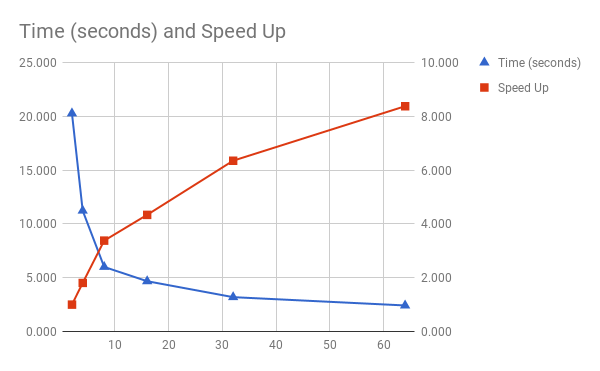
\includegraphics[width=0.48\textwidth]{figures/results/time.png}
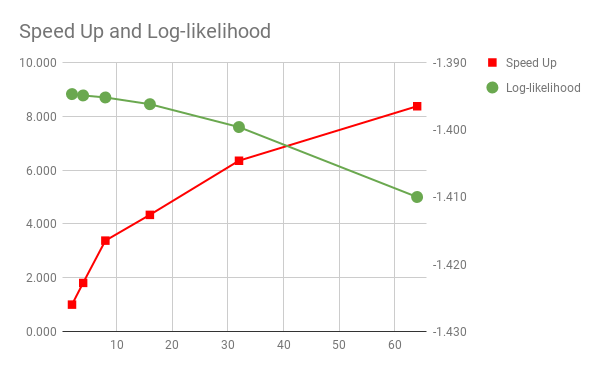
\includegraphics[width=0.48\textwidth]{figures/results/loglik.png}
\caption{
	Plots of results. The left one shows how the training time (per epoch) and speed-up change with the batch size, and the right one shows how (converged) log-likelihood changes with the batch size (with speed-up as a reference). As we can see, the speed-up increases sub-linearly, while the model performance decreases sharply at the beginning but saturates as the batch size gets larger. 
}
\label{fig:results}
\end{figure}
%

\subsection{Software Tool}
To implement this computational graph, we use Theano \citep{bastien-12-theano,bergstra-10-scipy}, a Python library that lets you to define, optimize, and evaluate mathematical expressions, especially ones with multi-dimensional arrays.

\subsection{Results}
In this section, we will analyze our experimental results. 

It took about 20 seconds for non-parallel implementation with stochastic gradient descent (SGD) to train on our simulated dataset for one epoch. We would like to investigate how much time it takes for our parallel implementation that enables mini-batch training on a GPU and how the parallel training affects the model performance, measured by {\em speed up} and {\em log-probability} after convergence respectively. The results are shown in \cref{tab:results}.

\subsection{Analysis}
As shown in \cref{tab:results} and \cref{fig:results}, we can conclude that:
\begin{itemize}
\item Our matrix formulation and implementation of Hawkes process dramatically increased the training speed. With a batch of size 64, the training time was cut about 90\% off, yielding a speed-up of 9. 
\item The performance slightly degrades with parallelism. With a batch of size 64, the log-likelihood was decreased by 2\%. 
\end{itemize}

Moreover, we can observe, in \cref{fig:results} that the speed-up is sub-linear, which means that there are factors against the parallelism in the training. We believe that the factors are: 
\begin{itemize}
\item Startup cost. Most of the startup cost would be data transportation between GPU and CPU and the associated GPU cores assignment. 
\item Interference. The same set of model weights are shared by all the sequences in one batch, which results in resource awaiting. Updating the model weights batch after batch causes synchronization barriers---e.g. one batch of data needs to be moved out of GPU at a time but some longer sequences take more time. 
\item Skew. First, as the GPU cores often work in groups of 32 or 64, the total number of data and operations may not be a multiple of 32 or 64. Thus when training one batch is split into small tasks, not all the tasks are of the same size and not all the tasks finish at the same time. 
\end{itemize}

Here are some ways to tackle these factors against parallelism:
\begin{itemize}
\item Startup cost. We can first move all the data onto the GPU, if the GPU memory is large enough, such that we would never need to worry about the CPU-GPU transportation. 
\item Interference. We can try to put sequences of same (or similar) lengths into the same batch, to reduce the synchronization barriers~\footnote{Though some batches would be significantly larger than the others because they have the longest sequences in the basket!}.
\item Skew. This is harder to deal with, but we believe that the skew can be reasonably reduced if we deliberately calibrate the data amount in each batch such that each small task on GPU can better fit a group of 32 or 64 cores. 
\end{itemize}

\section{Conclusion and Future Work}
In this project, we investigated how to train a Hawkes process in batches. We reconstructed the training objective in its matrix format, thus enabling representing the objective computation for all the sequences in one batch as a computational graph. This conversion enables usage of powerful scientific computing libraries like Theano and matrix-friendly computation devices like GPUs, so that the training speed is dramatically increased, without sacrificing much performance. 

However, we could not manage to investigate how it helps (or hurts) to train in parallel with multiple GPUs (split either model weights or training sequences onto different devices) and this might be done in the future. 

\bibliography{neural-hawkes}
%\bibliographystyle{plain}
%\bibliographystyle{icml2016}
\bibliographystyle{plainnat}

\clearpage
\appendix
\appendixpage

\section{Likelihood Function}
\label{sec:likelihood}

\subsection{Likelihood For Point Processes}\label{sec:lik}
For the proposed models, given complete observations of an event stream over the time interval $[0,T]$, the log-likelihood of the parameters turns out to be given by the simple formula shown in \cref{sec:algo}.  We start by giving the full derivation of that formula, repeated here:
\begin{equation*}
    \ell = \sum_{i: t_i\leq T} \log \lambda_{k_i}(t_i) - \underbrace{\int_{t=0}^{T} \lambda(t) dt}_{\text{call this }\Lambda} \tag{\ref{eqn:loglik}}
\end{equation*}

First, we define $N(t) = |\{h: t_h \leq t\}|$ to be the count of events (of any type) preceding time $t$. So given the past history $\mathcal{H}_i$, the number of events in $(t_{i-1},t]$ is denoted as $\Delta N(t_{i-1},t) \defeq N(t)-N(t_{i-1})$.  Let $T_i > t_{i-1}$ be the random variable of the next event time and let $K_{i+1}$ be the random variable of the next event type.  The cumulative distribution function and probability density function of $T_i$ (conditioned on $\mathcal{H}_i$) are given by:
\begin{subequations} \label{eqn:nonhomo_F}
\begin{align}
	F(t)
	&= P(T_i \leq t) = 1-P(T_i > t) \\
	&= 1- P(\Delta N(t_{i-1},t)=0) \\
	&= 1- \exp \left( -\int_{t_{i-1}}^{t} \lambda(s) ds \right) \\
	&= 1- \exp \left( \Lambda(t_{i-1}) - \Lambda(t) \right) \\
	f(t)
	&= \exp \left( \Lambda(t_{i-1}) - \Lambda(t) \right) \lambda(t)
\end{align}
\end{subequations}
where \mbox{$\Lambda(t)=\int_{0}^{t} \lambda(s)ds$} and \mbox{$\lambda(t)=\sum_{k=1}^K \lambda_k(t)$}.

Moreover, given the past history $\mathcal{H}_i$ and the next event time $t_i$, the distribution of $k_i$ is given by:
\begin{equation}
    P(K_i=k_i \mid t_i) = \frac{\lambda_{k_i} (t_i)}{\lambda(t_i)}
\end{equation}

Therefore, we can derive the likelihood function as follows:
\begin{subequations} \label{eqn:likelihood_nonhomo}
\begin{align}
    \mathcal{L}
    &= \prod_{i: t_i\leq T}{\mathcal{L}_i} = \prod_{t_i\leq T}\{{f(t_i ) P(K_i=k_i \mid t_i)} \} \\
    &= \prod_{i: t_i\leq T} \{ \exp \left( \Lambda(t_{i-1}) - \Lambda(t_i) \right) \lambda_{k_i}(t_i) \}
\end{align}
\end{subequations}
and
\begin{subequations} \label{eqn:log-likelihood_nohomo}
\begin{align}
    \ell
    &\defeq \log \mathcal{L} \\
    &= \sum_{i: t_i\leq T} \log \lambda_{k_i}(t_i) - \sum_{i:t_i\leq T} \left( \Lambda(t_i)-\Lambda(t_{i-1}) \right) \\
    &= \sum_{i: t_i\leq T} \log \lambda_{k_i}(t_i) - \Lambda(T) \\
    &= \sum_{i: t_i\leq T} \log \lambda_{k_i}(t_i) - \int_{t=0}^{T} \lambda(t) dt
\end{align}
\end{subequations}

%We need to notice that $\lambda_{k}(t)$ is left-continuous at $t_{i}$, so we denote in this case that \mbox{$\lambda_{k}(t_{i}^{+}) = \lim_{t \to t_{i}, t > t_{i}} \lambda_{k}(t)$}.

\subsection{Likelihood For a Hawkes Process}\label{sec:likhawkes}
To further derive the log-likelihood function for a Hawkes process, we need to consider the integral term in \cref{eqn:loglik}, which could be expanded by plugging in \cref{eqn:hawkes}:
\begin{subequations}
\begin{align}
\int_{t=0}^{T} \lambda(t)dt 
&= T \sum_{k=1}^{K} \mu_k + \sum_{k=1}^{K} \int_{t=0}^{T} \sum_{h:t_h < t} \frac{\alpha_{k_h,k}}{\delta_{k_h,k}} \exp(-\delta_{k_h,k}(t-t_h)) d(\delta_{k_h,k}(t-t_h))\\
&= T \sum_{k=1}^{K} \mu_k + \sum_{k=1}^{K} \int_{t=0}^{T} \sum_{h:t_h < t} \frac{\alpha_{k_h,k}}{\delta_{k_h,k}} \exp(-\delta_{k_h,k}(t-t_h)) d(\delta_{k_h,k}(t-t_h))\\
&= T \sum_{k=1}^{K} \mu_k + \sum_{k=1}^{K} \sum_{i=1}^{I} \frac{\alpha_{k_i,k}}{\delta_{k_i,k}} \int_{t=t_i}^{T} \exp(-\delta_{k_i,k}(t-t_i)) d(\delta_{k_i,k}(t-t_i))\\
&= T \sum_{k=1}^{K} \mu_k - \sum_{k=1}^{K} \sum_{i=1}^{I} \frac{\alpha_{k_i,k}}{\delta_{k_i,k}} \int_{t=t_i}^{T} \exp(-\delta_{k_i,k}(t-t_i)) d(-\delta_{k_i,k}(t-t_i))\\
&= T \sum_{k=1}^{K} \mu_k - \sum_{k=1}^{K} \sum_{i=1}^{I} \frac{\alpha_{k_i,k}}{\delta_{k_i,k}} \exp(-\delta_{k_i,k}(t-t_i)) |_{t_i}^{T}\\
&= T \sum_{k=1}^{K} \mu_k - \sum_{k=1}^{K} \sum_{i=1}^{I} \frac{\alpha_{k_i,k}}{\delta_{k_i,k}} (\exp(-\delta_{k_i,k}(T-t_i)) - 1 )\\
&= T \sum_{k=1}^{K} \mu_k + \sum_{k=1}^{K} \sum_{i=1}^{I} \frac{\alpha_{k_i,k}}{\delta_{k_i,k}} ( 1 - \exp(-\delta_{k_i,k}(T-t_i)) )
\end{align}
\end{subequations}

\section{Thinning Algorithm for Sampling Sequences}
\label{sec:thinning}

If we wish to draw sequences from a Hawkes process, we can adopt the thinning algorithm~\citep{lewis-79-sim,liniger-09-hawkes} that is commonly used for the multivariate Hawkes process, as shown in~\cref{alg:thinning}.  We explain the algorithm here and illustrate its conception in \cref{fig:thinning}.

Suppose we have already sampled the first $i-1$ events.
The $K$ event types are now in a race to see who generates the next event. How do we conduct the race?  For each event type $k$, let the function $\lambda_k^i: (t_{i-1},\infty) \rightarrow \Real_{\geq 0}$ map each time $t$ to the intensity $\lambda_k^i(t)$ that our model will define at time $t$
provided that event $i$ has not yet happened in the interval $(t_{i-1},t)$.  For each $k$ independently, we draw the time $t_{i,k}$ of the next event from the non-homogeneous Poisson process over $(t_{i-1},\infty)$ whose intensity function is $\lambda_k^i$.  We then take $t_i = \min_k t_{i,k}$ and $k_i = \argmin_k t_{i,k}$.  That is, we keep just the earliest of the $K$ events.  We cannot keep the rest because they are not correctly distributed according to the new intensities as updated by the earliest event.

But how do we draw the next event time $t_{i,k}$ from the non-homogeneous Poisson process given by $\lambda_k^i$?  Recall from \ref{sec:poisson_process} that a draw from such a point process is actually a whole {\em set} of times in $(t_{i-1},\infty)$: we will take $t_{i,k}$ to be the earliest of these.  In theory, this set is drawn by {\em independently} choosing at each time $t \in (t_{i-1},\infty)$, with infinitesimal probability proportional to $\lambda_k^i(t)$, whether an event occurs.  One could do this by {\em independently} applying rejection sampling at each time $t$: choose with larger probability $\lambda^*$ whether a ``proposed event'' occurs at time $t$, and if it does, accept the proposed event with probability only $\lambda_k^i(t)/{\lambda^*} \leq 1$. This is equivalent to simultanously drawing a set of proposed times from a {\em homogenous} Poisson process with constant rate $\lambda^*$, and then ``thinning'' that proposed set, as illustrated in \cref{fig:thinning}.   This approach helps because it is easy to draw from the homogenous process: the intervals between successive proposed events are IID $\Exp(\lambda^*)$, so it is easy to sample the events in sequence.  The inner {\bf repeat} loop in \cref{alg:thinning} lazily carries out just enough of this infinite homogenous draw from $\lambda^*$ to determine the time $t_{i,k}$ of the earliest {\em accepted} event, which is the earliest event in the non-homogeneous draw from $\lambda_k^i$, as desired.
% \cref{fig:thinning} is a conceptual illustration of an infinitely long sequence.

Finally, how do we construct the upper bound $\lambda^*$ on $\lambda_k^i$?
%\Cref{eqn:hawkes,eqn:hawkes_inhib,eqn:neural_hawkes} each
Recall that the excitation effect in Hawkes process is exponentially decaying, so the upper bound $\lambda^*$ is in fact $\lim_{t \rightarrow t_{i-1}}\lambda_{k}^i(t)$ with $t \in ( t_{i-1}, \infty)$. 

\begin{figure}
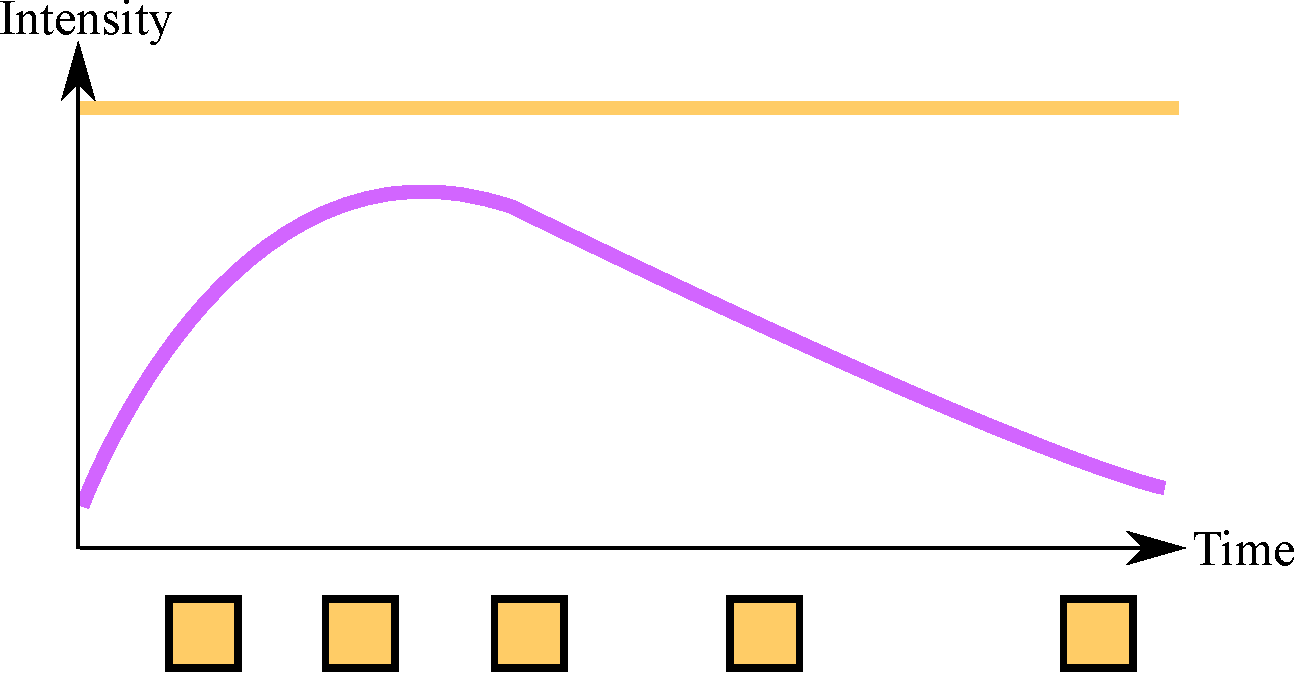
\includegraphics[width=0.32\linewidth]{./figures/thinning/1.pdf}
%\hfill
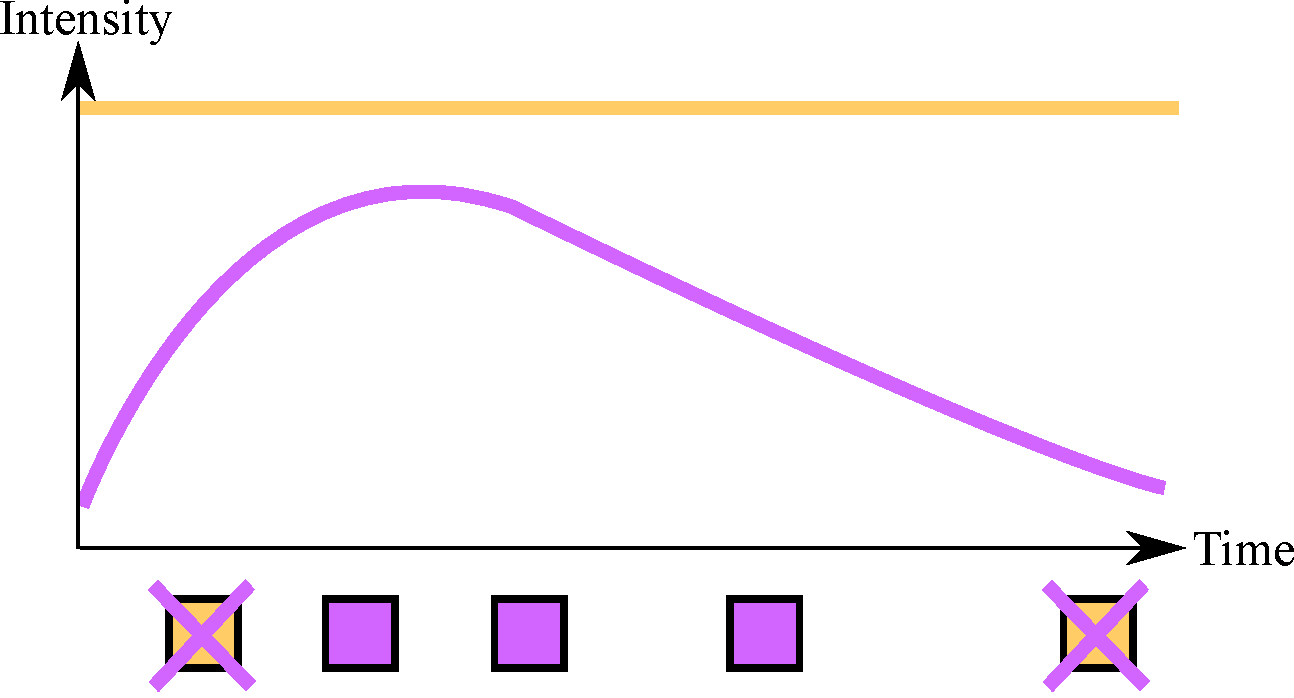
\includegraphics[width=0.32\linewidth]{./figures/thinning/2.pdf}
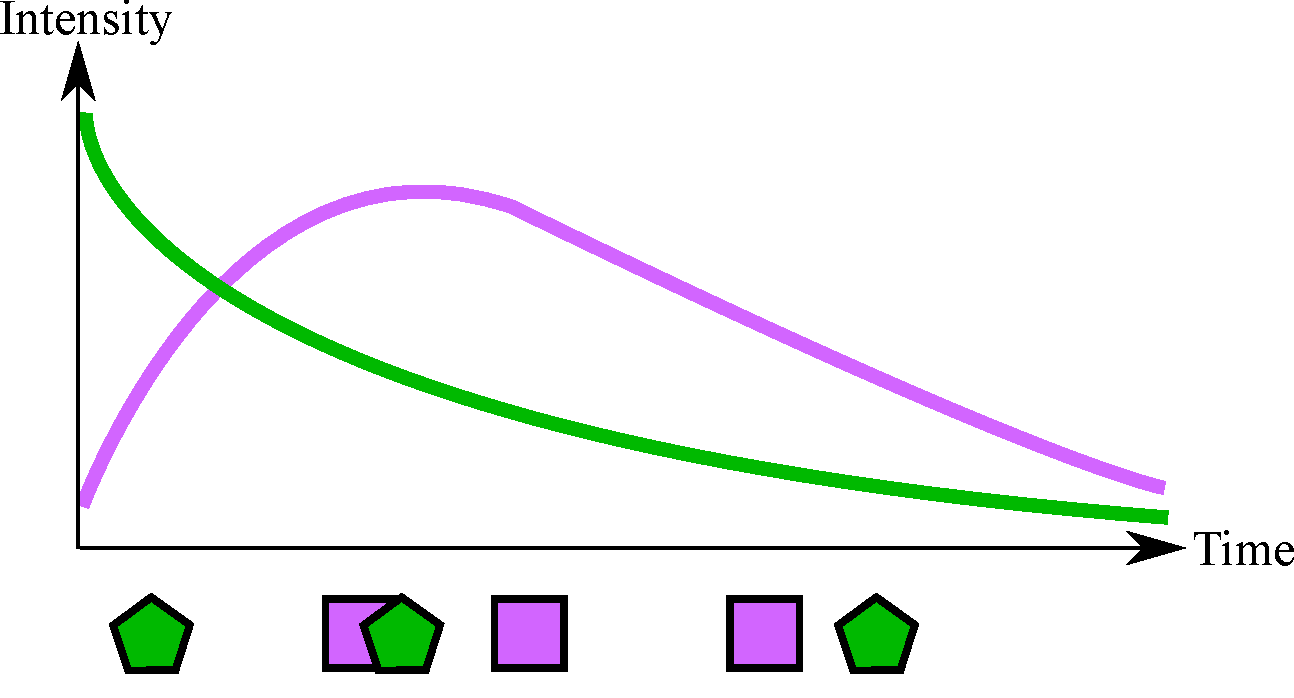
\includegraphics[width=0.32\linewidth]{./figures/thinning/3.pdf}
%\hfill
%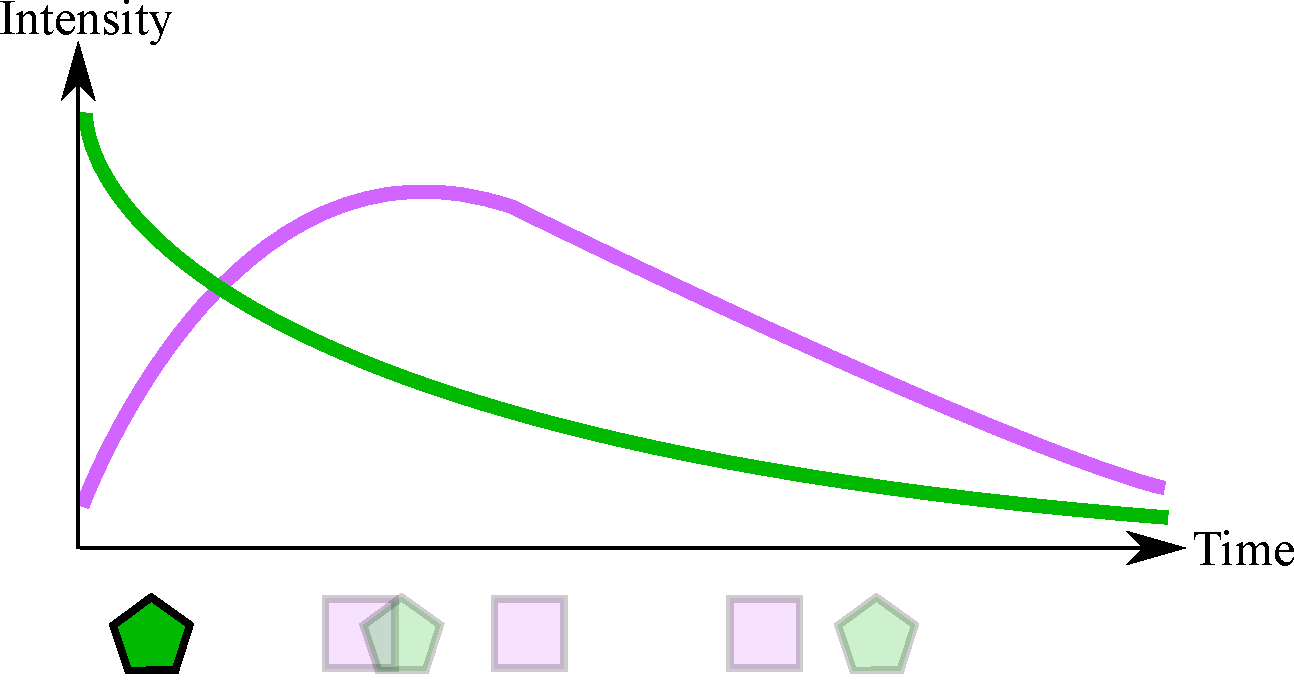
\includegraphics[width=0.48\linewidth]{./figures/thinning/4.pdf}
\caption{
Sampling the next event, where {gold} denotes proposed events, while purple and green denote two different types of events. The $x$ axis shows a prefix of the infinite interval $(t_{i-1,\infty})$.
In the first graph, {\em gold} events are proposed from a homogeneous Poisson process with intensity $\lambda^*$ (gold straight line). In the second graph, the purple curve $\lambda_1^i$ randomly accepts some of these gold events, with probability $\lambda_1^i(t) / \lambda^*$ for the event at time $t$; here it accepts three of the ones shown and rejects the others. In the third graph, the surviving type-1 events (purple squares) are interleaved with the surviving type-2 events (green pentagons). The next event is the earliest one among these surviving candidates.  In practice, these sequences are constructed lazily so that we find only the earliest surviving event of each type.  This is possible because the inter-arrival times between gold proposed events are distributed as $\text{Exp}(\lambda^*)$, making it straightforward to enumerate any finite prefix of a random infinite gold sequence.
}\label{fig:thinning}
\end{figure}

\begin{algorithm}[tb]
	\caption{Data Simulation (thinning algorithm)}
	\label{alg:thinning}
	\begin{algorithmic}
	\State {\bfseries Input:} interval $[0,T]$; model parameters
        \State $t_0\gets 0$; $i\gets 1$
	%\Repeat
		\While{$t_{i-1} < T$} \Comment{draw event $i$, as it might fall in [0,T]}
			\For{$k=1$ {\bfseries to} $K$} \Comment{draw ``next'' event of each type}
				\State find upper bound $\lambda^* \geq \lambda_k^i(t)$ for all $t \in (t_{i-1},\infty)$
				%\State For Hawkes process, $\lambda^*_{i,k}=\lambda_{i,k,0} = \lambda_{k}(t_{i-1}^{+} )$
				%\State For our models,
				%\State Set $t_{i,k,0} = t_{i-1}$,  $\lambda_{i,k,0} = \lambda_{k}(t_{i-1}^{+} )$ and $j=0$
				\State $t \gets t_{i-1}$
				%\State Set $\lambda_{i,k,0} = \lambda_{k}(t_{i-1}^{+} )$
					\Repeat
						%\State Sample $u_{1},u_{2} \sim \Uniform(0,1)$
						%\State $\tau_{i,k,j} = -\log u_1$
						\State draw $\Delta \sim \Exp(\lambda^*)$, $u \sim \Uniform(0,1)$
						\State $t \pluseq \Delta$ \Comment{time of next proposed event}
					\Until{$u\lambda^* \leq \lambda_k^i(t)$} \Comment{accept proposal with prob $\frac{\lambda_k^i(t)}{\lambda^*}$}
                                \State $t_{i,k} \gets t$
				%
			\EndFor
			\State $t_{i} \gets \min_{k} t_{i,k}$; $k_{i} \gets \argmin_{k} t_{i,k}$ \Comment{earliest event wins}
                        \State $i \gets i+1$
		\EndWhile
        \State \textbf{return} $(k_1,t_1),\ldots(k_{i-1},t_{i-1})$
\end{algorithmic}
\end{algorithm}

While \cref{alg:thinning} is classical and intuitive, we also implemented a more efficient variant.  Instead of drawing the next event from each of $K$ {\em different} non-homogeneous Poisson processes and keeping the earliest, we can construct a {\em single} non-homogenous Poisson process with aggregate intensity function $\lambda^i(t)=\sum_{k=1}^{K} \lambda^i_{k}(t)$ over $(t_{i-1},\infty)$.  An upper bound $\lambda^*$ on this aggregate function can be obtained by summing the upper bounds on the individual $\lambda^i_k$ functions.  We then use the thinning algorithm only to sample the next event time $t_i$ from this aggregate process $\lambda^i$.  Finally, we ``disaggregate'' by choosing $k_i$ from the distribution $p(k \mid t_i) = \lambda_{k}^i(t_i)/\lambda^i(t_i)$.\footnote{In practice, acceptance and disaggregation can be combined into a single step.  That is, each successive event $t$ proposed from the homogeneous $\text{Poisson}(\lambda^*)$ process is either kept as type $k$, with probability
  $\lambda_{k}^i(t)/\lambda^*$, or rejected, with probability $1 - \lambda^i(t)/\lambda^*$.
  If it is accepted, we have found our next event $(k_i,t_i)$.  If it is rejected, we increment $t$ by $\Delta \sim \text{Exp}(\lambda^*)$ to get the next proposed event.}
  This is equivalent to \cref{alg:thinning}.  In terms of \cref{fig:thinning}, this more efficient version enumerates a gold sequence that is the union of the $K$ gold sequences, and stops with the first accepted gold event.  Thus, whereas \cref{fig:thinning} had to propose two type-1 events in order to get the first accepted type-1 event (the leftmost purple event), the more efficient version would not have had to spend time proposing either of those, because an earlier proposed event (the leftmost green event) had already been accepted and determined to be of type 2.

\end{document}


% This document was modified from the file originally made available by
% Pat Langley and Andrea Danyluk for ICML-2K. This version was
% created by Lise Getoor and Tobias Scheffer, it was slightly modified
% from the 2010 version by Thorsten Joachims & Johannes Fuernkranz,
% slightly modified from the 2009 version by Kiri Wagstaff and
% Sam Roweis's 2008 version, which is slightly modified from
% Prasad Tadepalli's 2007 version which is a lightly
% changed version of the previous year's version by Andrew Moore,
% which was in turn edited from those of Kristian Kersting and
% Codrina Lauth. Alex Smola contributed to the algorithmic style files.
